\documentclass[10pt,a4paper]{article}
\usepackage[top=2.0cm,bottom=2.0cm,left=2.0cm,right=2.0cm]{geometry}
\usepackage{times}
\usepackage[T1]{fontenc}
\usepackage[utf8]{inputenc}
\usepackage{graphicx}
\usepackage{booktabs}
\usepackage{array}
\usepackage{tabularx}
\usepackage{enumitem}
\usepackage{hyperref}
\usepackage{xcolor}
\usepackage{titlesec}
\usepackage{parskip}
\usepackage{float}

\pagestyle{empty}
\titleformat{\section}{\normalfont\normalsize\bfseries\scshape\centering}{\thesection.}{0.5em}{}
\titleformat{\subsection}{\normalfont\normalsize\itshape}{\thesubsection.}{0.5em}{}
\hypersetup{colorlinks=true,linkcolor=black,urlcolor=blue,citecolor=black}

\begin{document}

\begin{titlepage}
\centering
\vspace*{2cm}
{\fontsize{24pt}{28pt}\selectfont\bfseries
COMPARATIVE ANALYSIS OF DEEP LEARNING\\[6pt]
ARCHITECTURES FOR SENTIMENT ANALYSIS\\[6pt]
OF MOVIE REVIEWS\par}
\vspace{1.5cm}
{\large Interim report on\\[4pt] Deep Learning Project\\[4pt] {[ICT-4442]}\par}
\vspace{2cm}
{\large\bfseries Submitted By\par}
\vspace{0.8cm}
{\fontsize{11pt}{14pt}\selectfont
Meesha Gupta (230953090)\\[4pt]
Ratul Jha (230953338)\\[4pt]
Harshavardhan Reddy (230953396)\\[4pt]
Kshitij Singh (230953460)\par}
\vfill

\includegraphics[width=0.25\textwidth]{figures/mit_logo.png}\\[12pt]
{\large\bfseries
SCHOOL OF COMPUTER ENGINEERING\\[4pt]
MANIPAL INSTITUTE OF TECHNOLOGY,\\[4pt]
MANIPAL ACADEMY OF HIGHER EDUCATION\par}
\vspace{1cm}
{\large October 2026\par}
\end{titlepage}

\begin{center}
{\Large\bfseries\scshape Part B : Interim Report}\\[6pt]
{\small Phase 2 - Late submission draft}
\end{center}
\vspace{0.5cm}
\noindent\textbf{Team No. and Names (with Registration Numbers):}\\[4pt]
\begin{tabular}{@{}ll@{}}
1. & Meesha Gupta (230953090) \\
2. & Ratul Jha (230953338) \\
3. & Harshavardhan Reddy (230953396) \\
4. & Kshitij Singh (230953460) \\
\end{tabular}

\vspace{0.5cm}
\noindent\textbf{Title of the Project:}\\[4pt]
Comparative Analysis of Deep Learning Architectures for Sentiment Analysis of Movie Reviews

\vspace{0.5cm}
\noindent\textbf{GitHub Repository Link:}\\[4pt]
\url{https://github.com/HarshavardhanReddy585/imdb-sentiment-analysis-ict4442}

\section{Literature Review}
The literature review covers feed-forward, convolutional, recurrent, and pretrained Transformer architectures. Table~\ref{tab:lit} summarises the ten papers reviewed and their relevance to the proposed comparison.

\begin{table}[H]
\caption{Literature Review Summary}\label{tab:lit}
\centering\small\renewcommand{\arraystretch}{1.2}
\begin{tabularx}{\textwidth}{>{\raggedright\arraybackslash}p{2.5cm} >{\raggedright\arraybackslash}p{2.3cm} >{\raggedright\arraybackslash}p{1.8cm} >{\raggedright\arraybackslash}p{2.7cm} X}
\toprule
\textbf{Paper} & \textbf{Method} & \textbf{Dataset} & \textbf{Key result} & \textbf{Relevance} \\
\midrule
Maas et al. (2011) [1] & Sentiment-aware word vectors & IMDb 50k & Established a labelled and unlabelled movie-review benchmark. & Defines the dataset and benchmark used here. \\
\midrule
Kim (2014) [2] & 1D CNN with multiple filter widths & Sentence classification & Local phrase filters perform strongly with a simple architecture. & Motivates the multi-width CNN. \\
\midrule
Hochreiter and Schmidhuber (1997) [3] & LSTM recurrent units & Sequence modelling & Gated memory addresses vanishing-gradient limitations. & Provides the recurrent foundation for BiLSTM. \\
\midrule
Schuster and Paliwal (1997) [4] & Bidirectional RNN & Speech sequences & Processing both directions improves sequence representation. & Supports bidirectional text modelling. \\
\midrule
Mikolov et al. (2013) [5] & Word2Vec representations & Large text corpora & Distributed embeddings encode useful lexical regularities. & Informs learned word representations. \\
\midrule
Peters et al. (2018) [6] & ELMo contextual representations & Multiple NLP tasks & Contextual embeddings transfer across tasks. & Connects static embeddings to contextual models. \\
\midrule
Vaswani et al. (2017) [7] & Transformer self-attention & Translation tasks & Self-attention models token dependencies without recurrence. & Architectural basis for DistilBERT. \\
\midrule
Devlin et al. (2019) [8] & BERT pretraining and fine-tuning & GLUE and SQuAD & Bidirectional pretraining improved many language tasks. & Establishes the pretrained reference point. \\
\midrule
Sanh et al. (2019) [9] & DistilBERT knowledge distillation & Language understanding & A smaller model retains much of BERT's capability. & Specifies the planned Transformer comparison. \\
\midrule
Howard and Ruder (2018) [10] & ULMFiT & Text classification & Transfer learning and fine-tuning improve classification. & Supports controlled pretrained-model evaluation. \\
\bottomrule
\end{tabularx}
\end{table}

\section{Dataset Acquisition \& Preprocessing}
\subsection*{Dataset}
The project uses the IMDb Large Movie Review Dataset introduced by Maas et al. [1]. It contains 50,000 labelled reviews, balanced between positive and negative classes, with 25,000 official training reviews and 25,000 official test reviews. The archive is downloaded locally and excluded from Git.

\subsection*{Data Splits}
The official training directory is shuffled with seed 42 and divided into 80\% training and 20\% validation. The official test directory remains untouched until evaluation. The verified MLP and CNN full-protocol runs use 20,000 training, 5,000 validation, and 25,000 test reviews and were trained for three epochs. The BiLSTM CPU smoke run uses 800, 200, and 200 reviews.

\subsection*{Preprocessing Pipeline}
\begin{enumerate}[nosep]
\item Read reviews from the official \texttt{train/neg}, \texttt{train/pos}, \texttt{test/neg}, and \texttt{test/pos} folders.
\item Lowercase text and tokenize alphabetic words plus apostrophes, retaining sentiment-bearing terms such as ``not''.
\item Build vocabulary from the training partition only. MLP/CNN runs retain the 20,000 most frequent tokens plus padding and unknown tokens; the BiLSTM smoke run uses a 12,000-token vocabulary.
\item Encode, pad, and truncate reviews deterministically. MLP/CNN use 512 tokens; the CPU BiLSTM smoke run uses 40 tokens.
\item Use the same seed, split policy, and accuracy, precision, recall, F1, and confusion-matrix metrics for model evaluation.
\end{enumerate}

\section{Models Implemented So Far}
The repository contains reproducible PyTorch implementations for the MLP, 1D-CNN, and BiLSTM. DistilBERT remains pending and is not represented by fabricated results.

\subsection*{A. Multi-Layer Perceptron (MLP)}
The MLP uses a learned embedding layer, masked average pooling, a 64-unit ReLU hidden layer, dropout, and a binary classifier. It was trained for three epochs on the full 20,000/5,000/25,000 protocol. Validation accuracy was 88.50\% with F1 = 0.884; test accuracy was 86.31\% with F1 = 0.858.

\subsection*{B. 1D Convolutional Neural Network (1D-CNN)}
The CNN uses a learned embedding layer and parallel Conv1D branches with kernel widths 3, 4, and 5, followed by max pooling and classification. On the full 20,000/5,000/25,000 protocol, validation accuracy was 79.64\% with F1 = 0.783; test accuracy was 79.53\% with F1 = 0.780. The remaining tuning focus is improving the balance between precision and recall.

\subsection*{C. Bidirectional LSTM (BiLSTM)}
The BiLSTM uses an embedding layer, a bidirectional LSTM, concatenated final hidden states, and a binary classifier. The CPU smoke run on 800 training, 200 validation, and 200 test reviews achieved 46.5\% validation accuracy and 51.0\% test accuracy. These values are preliminary and require a larger rerun.

\subsection*{D. DistilBERT}
DistilBERT is the fourth proposed architecture. Its implementation and metrics are not yet evidenced in the canonical repository, so its status is recorded as pending.

\subsection*{Interim Results and Visual Evidence}
The numerical evidence below is generated from the JSON files in \texttt{results/}. The accompanying notebook \texttt{notebooks/interim\_results\_visualization.ipynb} loads those files and displays the same figures. The MLP and CNN results are full-protocol results; the BiLSTM value is explicitly labelled as smoke evidence.

\begin{table}[H]
\caption{Verified interim test results}
\centering\small\renewcommand{\arraystretch}{1.25}
\begin{tabularx}{\textwidth}{l c c c c X}
\toprule
\textbf{Model} & \textbf{Train} & \textbf{Validation} & \textbf{Test} & \textbf{Test F1} & \textbf{Evidence status} \\
\midrule
MLP & 20,000 & 5,000 & 25,000 & 0.858 & Full three-epoch protocol completed. \\
\midrule
1D-CNN & 20,000 & 5,000 & 25,000 & 0.780 & Full three-epoch protocol completed. \\
\midrule
BiLSTM & 800 & 200 & 200 & 0.372 & Harshavardhan's CPU smoke evidence; model in progress. \\
\bottomrule
\end{tabularx}
\end{table}

\begin{figure}[H]
\centering
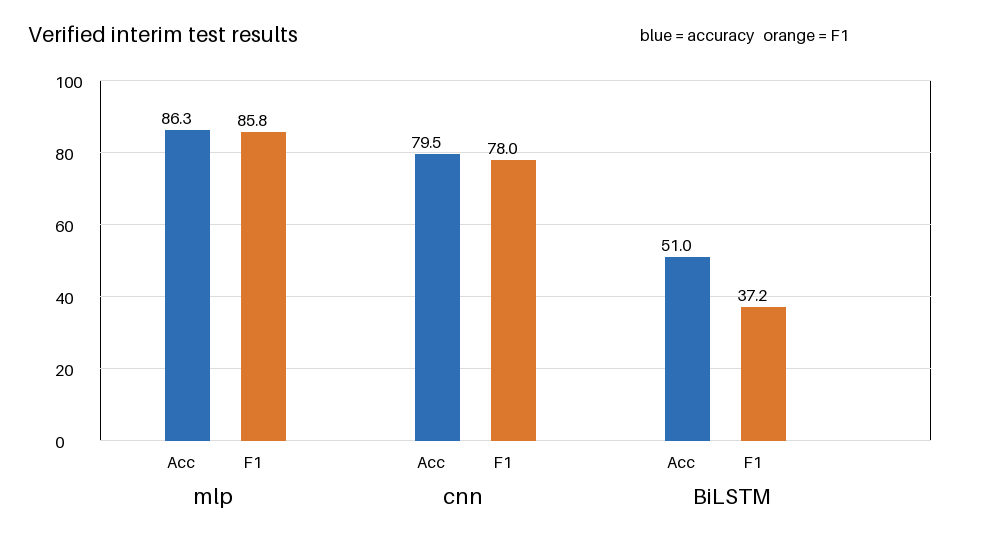
\includegraphics[width=0.78\textwidth]{figures/verified_test_comparison.png}
\caption{Test accuracy and F1 score from the verified interim JSON metrics.}
\label{fig:testcomparison}
\end{figure}

\begin{figure}[H]
\centering
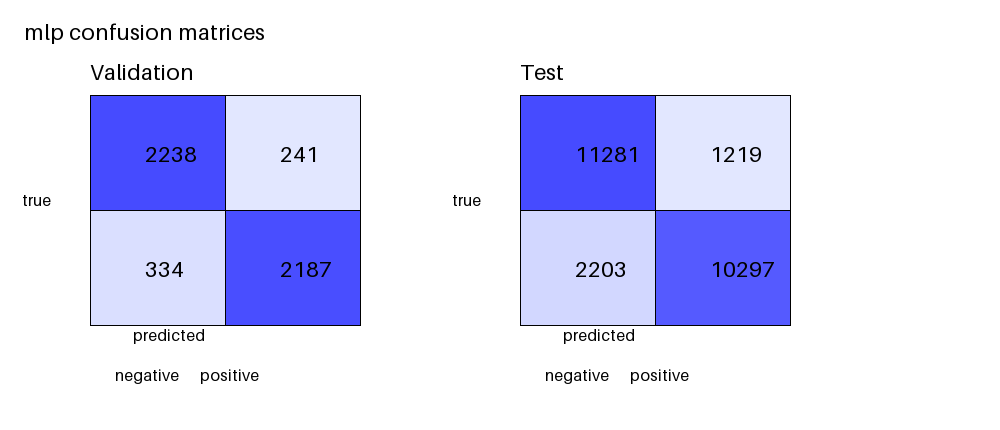
\includegraphics[width=0.98\textwidth]{figures/mlp_confusion_matrices.png}
\caption{MLP validation and test confusion matrices from the full-protocol run.}
\label{fig:mlpcm}
\end{figure}

\begin{figure}[H]
\centering
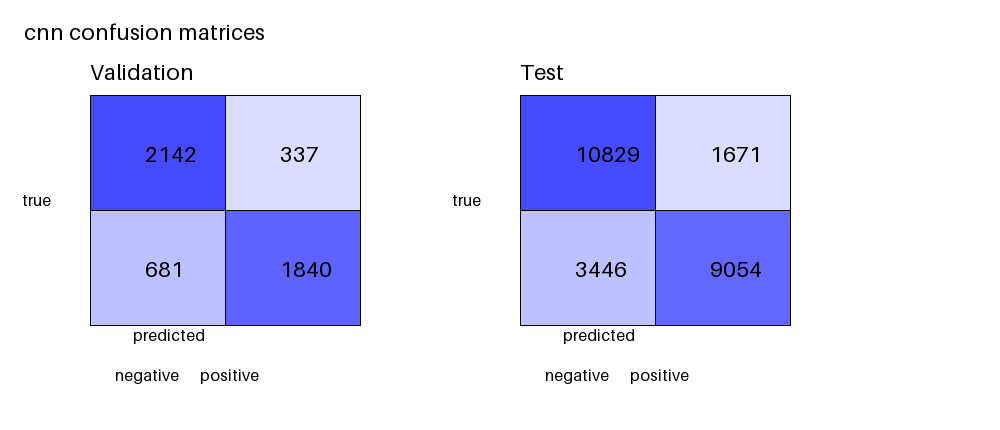
\includegraphics[width=0.98\textwidth]{figures/cnn_confusion_matrices.png}
\caption{CNN validation and test confusion matrices from the completed full-protocol run.}
\label{fig:cnncm}
\end{figure}

\begin{figure}[H]
\centering
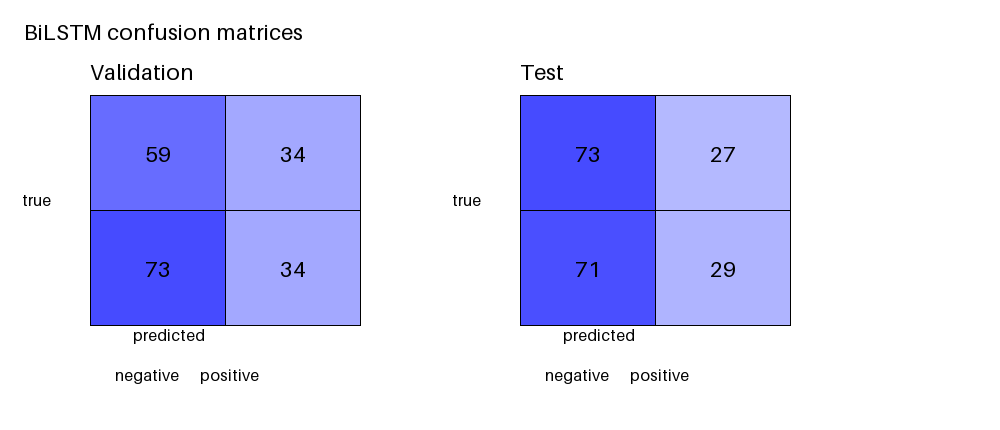
\includegraphics[width=0.98\textwidth]{figures/bilstm_confusion_matrices.png}
\caption{BiLSTM validation and test confusion matrices from the CPU smoke run.}
\label{fig:bilstmcm}
\end{figure}

\begin{table}[H]
\caption{Models Implemented - Status and Preliminary Results}
\centering\small\renewcommand{\arraystretch}{1.25}
\begin{tabularx}{\textwidth}{l l l >{\raggedright\arraybackslash}p{3cm} X}
\toprule
\textbf{Model} & \textbf{Owner} & \textbf{Status} & \textbf{Preliminary metric} & \textbf{Notes} \\
\midrule
MLP & Kshitij Singh & Complete & Val Acc: 88.50\%\\Val F1: 0.884 & Full 20,000/5,000/25,000 run; 512-token inputs. \\
\midrule
1D-CNN & Ratul Jha & Complete & Val Acc: 79.64\%\\Test Acc: 79.53\% & Full 20,000/5,000/25,000 run; evidence available. \\
\midrule
BiLSTM & Harshavardhan Reddy & Smoke evidence & Val Acc: 46.5\%\\Test Acc: 51.0\% & CPU smoke run; larger rerun pending. \\
\midrule
DistilBERT & Meesha Gupta & Pending & Pending & No local metric is claimed. \\
\bottomrule
\end{tabularx}
\end{table}

\section{Individual Contribution Log (to date)}
\begin{table}[H]
\caption{Individual Contribution Log}
\centering\small\renewcommand{\arraystretch}{1.3}
\begin{tabularx}{\textwidth}{l l >{\raggedright\arraybackslash}X l}
\toprule
\textbf{Member} & \textbf{Reg. No.} & \textbf{Task status recorded} & \textbf{Signature} \\
\midrule
Meesha Gupta & 230953090 & DistilBERT ownership recorded; implementation and evidence pending verification. & \\
\midrule
Ratul Jha & 230953338 & 1D-CNN ownership recorded; repository invitation pending acceptance; contribution to be verified. & \\
\midrule
Harshavardhan Reddy & 230953396 & Main contributor: report integration, preprocessing, experiment orchestration, result visualisation, and BiLSTM implementation in progress. & \\
\midrule
Kshitij Singh & 230953460 & MLP ownership recorded; contribution to be verified. & \\
\bottomrule
\end{tabularx}
\end{table}

\noindent\textbf{Repository evidence:} The canonical private repository contains the source code, generated metrics, and this report. Signatures and member-specific claims must be obtained honestly; they must not be simulated.

\section{Risk / Plan for Remaining Work}
\subsection*{Remaining Work}
\begin{enumerate}[nosep]
\item Implement and evaluate DistilBERT using the common dataset protocol.
\item Rerun BiLSTM and the scratch models at the full 20,000/5,000/25,000 split when compute permits.
\item Generate learning curves, ROC curves, confusion matrices, and systematic error analysis.
\item Complete the final Part C report, signed contribution statements, and presentation material.
\end{enumerate}

\subsection*{Expected Challenges}
\begin{itemize}[nosep]
\item CPU runtime may limit full-scale recurrent and Transformer training; staged runs and saved metrics will be used.
\item The CNN still requires tuning to improve the balance between precision and recall.
\item A fair comparison requires a frozen split, seed, metric set, and explicit documentation of tokenizer differences.
\item Late submission may require faculty approval; the report and repository evidence are being prepared immediately.
\end{itemize}

\subsection*{Timeline to Final Submission}
\begin{table}[H]
\centering\small\renewcommand{\arraystretch}{1.2}
\begin{tabularx}{\textwidth}{c X c}
\toprule
\textbf{No.} & \textbf{Milestone} & \textbf{Target} \\
\midrule
1 & DistilBERT implementation and four-model evaluation & 10 Oct 2026 \\
2 & Comparative metrics, figures, and confusion matrices & 18 Oct 2026 \\
3 & Error analysis and final Part C report & 27 Oct 2026 \\
4 & Slides, rehearsal, signatures, and final code push & 31 Oct 2026 \\
\bottomrule
\end{tabularx}
\end{table}

\vspace{0.5cm}\noindent\rule{\textwidth}{0.4pt}
\vspace{0.3cm}\noindent{\small\scshape References}
\begin{enumerate}[label={[$\arabic*]}, nosep, leftmargin=1.5em, font=\small]
\item A. L. Maas et al., ``Learning Word Vectors for Sentiment Analysis,'' ACL-HLT, 2011.
\item Y. Kim, ``Convolutional Neural Networks for Sentence Classification,'' EMNLP, 2014.
\item S. Hochreiter and J. Schmidhuber, ``Long Short-Term Memory,'' Neural Computation, 1997.
\item M. Schuster and K. K. Paliwal, ``Bidirectional Recurrent Neural Networks,'' IEEE TSP, 1997.
\item T. Mikolov et al., ``Efficient Estimation of Word Representations in Vector Space,'' arXiv:1301.3781, 2013.
\item M. E. Peters et al., ``Deep Contextualized Word Representations,'' NAACL, 2018.
\item A. Vaswani et al., ``Attention Is All You Need,'' NeurIPS, 2017.
\item J. Devlin et al., ``BERT: Pre-training of Deep Bidirectional Transformers for Language Understanding,'' NAACL-HLT, 2019.
\item V. Sanh et al., ``DistilBERT, a Distilled Version of BERT,'' NeurIPS EMC2 Workshop, 2019.
\item J. Howard and S. Ruder, ``Universal Language Model Fine-tuning for Text Classification,'' ACL, 2018.
\end{enumerate}

\end{document}
